\section{Data set}

\subsection{Subjects and set-up}
\label{subsec:setup}

Six female subjects, Italian mothertongue, were recorded while uttering
Italian words and pseudo-words. Words were mainly stress-initial, e.g.,
/matto/, /nome/, /strada/ (mad, name, road), and were chosen in order
to have consonants both at the beginning and in the middle of
words, followed by different vowels and consonants.
The data recording setup includes a \emph{Laryngograph Microprocessor}
device (Laryngograph Ltd., London \cite{...}) to gather the speech audio
signal and the electroglottographic (EGG) signal at $16$KHz sampling
rate; and an AG500 electromagnetic articulograph (Carstens Medizinelektronik
GmbH, Germany \cite{...}) to record at a sampling rate of $200$Hz the
3D positions of a set of sensors glued on the tongue, lips and front teeth
during speech production. A full description of the acquisition set-up and
the obtained database can be found in \cite{tavella}.

The subset used in this work comprises $77$ words containing /b/, /p/,
/d/ or /t/. These consonants were chosen because \textbf{GIUSTIFICAZIONE
PRECISA: letteratura sulle stop consonant, esperimenti neuroscientifici
sulla loro produzione e percezione.}

\subsection{Segmentation}
\label{subsec:segm}

Traditionally \cite{...}, the audio speech signal is segmented with a
fixed-length Hamming window, usually 20ms. long. The resulting sequence
is then analysed in the frequency or cepstral domain \cite{...} and the
resulting coefficients are used as features for a classification system.
This approach neglects the qualitative overall characteristics of the
phoneme being uttered: depending on the speed of the speech, a consonant
can have different lengths and, by using the above approach, global
information about it is lost (see \cite{...}, where this approach is
dubbed "beads-on-a-string"). Nevertheless, as far as we know, there is
so far no widely accepted alternative method for speech segmentation,
if the audio signal is the only one available.

An alternative way --- the one we actually pursue --- is that of defining
the length of a phoneme in terms of the phonetic gesture that produced
it. The audio signal is, therefore, segmented according to the motor
invariant chosen to represent the associated phonetic gesture.
A qualitative examination of the synchronised audio and motor
signals obtained from utterances of /b/, /p/, /d/ and /t/
by different speakers indicates that common patterns can
actually be found in the behaviour of the related articulators.
For instance, as is apparent from Figure \ref{fig:isdView}, 
recurring shapes of the lips opening velocity and acceleration appear
when both /ba/ and /bufalo/ are considered, even when uttered by different
speakers. The same patterns can be observed when other words containing
/b/ and /p/ are considered, both when the phoneme appears at the beginning
or inside a word, and regardless of the phoneme appearing immediately after.

\begin{figure*}[t] \centering
  \begin{tabular}{c}
    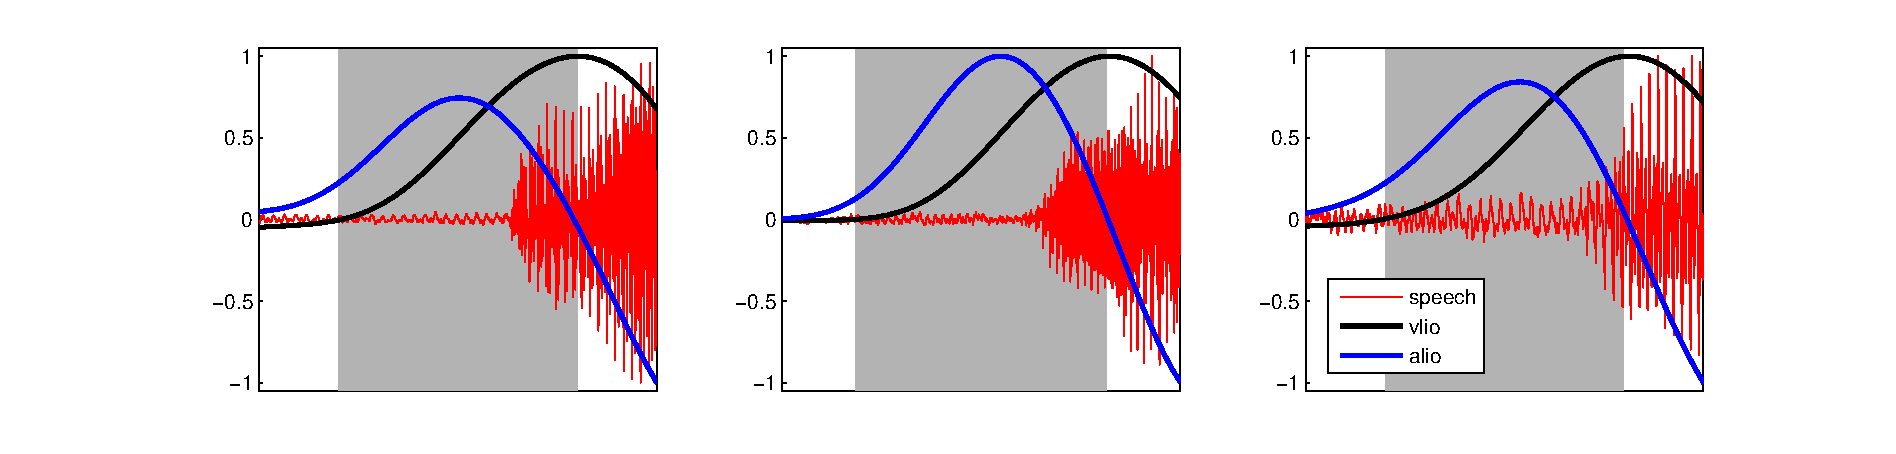
\includegraphics[width=\textwidth]{figs/figSamples} \\
  \end{tabular}
  \caption{the speech signal and motor trajectories of lips opening
    velocity (\vlio) and acceleration (\alio) during utterances containing /b/.
    Left to right: /ba/, subject $5$; /ba/, subject $2$; and /bufalo/, subject $5$.
    The gray zone denotes the detected start and ending of the plosion. All signals
    are normalised over the indicated time frame, for visualisation purposes.}
  \label{fig:isdView}
\end{figure*}

These observations visually confirm everyday experience and as well
basic definitions of stop consonants, found in any physiology textbook.
The following motor invariants are then defined and associated to the
consonants under examination:

\begin{enumerate}

  \item
    Let $s_1(t)$ and $s_2(t)$ be the signals associated
    with sensors placed on two phonetic actuators (e.g., the upper and
    lower lips), and $\delta(t) = ||s_1(t)-s_2(t)||$ be their
    Euclidean distance. Then, a plosion is defined as the interval
    between two instants $t_{start}$ and $t_{end}$ such that
    $\dot{\delta}(t_{start}) = 0 $ and $\ddot{\delta}(t_{start}) > 0$,
    and $\dot{\delta}(t_{end}) > 0 $ and $\ddot{\delta}(t_{end}) = 0$.

  \item For /b/ and /p/, the sensors on the upper and lower
    lip are considered for $s_1(t)$ and $s_2(t)$, whereas for /d/ and /t/
    those on the tongue tip and upper teeth are. In turn, the associated
    distances will be denoted as \lio\ (lips opening) and \ttu\
    (tongue tip - upper teeth distance).    

  \item To discriminate /b/ and /d/ from /p/ and /t/, the average of the
    voicing signal over the duration of the phoneme is considered. The
    voicing signal \cite{...} is derived from the EGG signal and indicates
    whether the vocal folds are activate.

\end{enumerate}

Condition $(1)$ physically defines a plosion: e.g., considering \lio, $t_{start}$
is just before opening the mouth and $t_{end}$ is at maximum velocity, just
before decelerating; condition $(2)$ selects an appropriate pair
of articulators needed for the phoneme under consideration;
condition $(3)$ discriminates voiced from voiceless consonants. This schema matches
the basic taxonomy of the consonants we are interested in, that is, plosive
bilabials (/b/, /p/) versus dentals (/d/, /t/) and voiced (/b/, /d/) versus
voiceless (/p/, /t/). In Figure \ref{fig:isdView} for example, the gray zone
indicates the start and ending of the invariants, gathered according to
condition $(1)$.

The segmentation is then carried out semi-automatically: for each
utterance, all sequences matching conditions $(1)$---$(3)$ are displayed and the
associated speech is played, so that the experimenter can choose whether the
sequence is a correct guess or it is a false positive. In this experiment we only
monitor \lio\ and \ttu, so that false positives appear, e.g., when considering
/ts/ and /dz/. This is why, at this stage, a completely automatic segmentation
cannot be enforced. If the sequence is accepted, it is labelled
with the associated consonant, the speaker, and the
coarticulating phoneme. For example, from the word /bronzo/ (bronze) a /b/
sequence is extracted, and the letter "r" is stored as the coarticulating phoneme.
By hearing the obtained sequences, one notices that they contain some of the
coarticulating sound, but this is inevitable according to the MTS \cite{...}. 

This way, from the original $77$ words and pseudowords, a total
of $1165$ audio/motor sequences are extracted, with a length of $121.43 \pm 41.63$
milliseconds (mean $\pm$ one standard deviation).
%In turn, 
%
%\begin{itemize}
%
%  \item $292$ /b/, $305$ /p/, $60$ /d/ and $508$ /t/;
%
%  \item $213,151,158,230,242,171$ for subjects $1,\ldots,6$;
%
%  \item $354,62,100,379,167,71,32$ for each coarticulating phoneme
%    /a/, /e/, /i/, /o/, /u/, /r/ and /s/.
%
%\end{itemize}
%
%Notice that no distinction is made whether the consonant is at the beginning
%of an utterance (e.g., /b/ in /baffo/, moustache) or in the middle of
%it (e.g., /d/ in /strada/, \emph{road}).
